\documentclass[12pt]{article}
\usepackage{titling}
\usepackage{graphicx}
\usepackage[top=1in, bottom=1.5in, left=1in, right=1in]{geometry}

\title{Designing a Hobbiest Embedded Microcontroller Laboratory}
\author{Team 12 \\ Stuart Larsen \ \ \ \ \   Troy Drabek \\ Keegan Larkin \ \ \ \ \   Adam Funkenbusch \\ Andrew Wallis }
\date{\today}

\begin{document}
\maketitle
\thispagestyle{empty}

\pagebreak


\section{Team Members}
\begin{center}
  \begin{tabular}{  l | p{8cm} | l }
    Name & Position & Email \\
    \hline
    Stuart Larsen & Project Lead & sclarsen@mtu.edu \\ 
    Troy Drabek & Expert in Microcontroller Design & tqdrabek@mtu.edu \\
    Keegan Larkin & Expert in Fabrication and Synthsis of Macro Quantum Electrodynamic Embedded Devices  & kjlarkin@mtu.edu \\
    Andrew Wallis & Resident Process Failure Mode and Effects Analysis Guru & amwallis@mtu.edu \\
    Adam Funkenbusch & Expert wire cutter & aefunken@mtu.edu \\
  \end{tabular}
\end{center}

\section{Overview and Orientation}
  The current design for the laboratory entails multiple lab benches configured to ease in the development of software systems for popular microcontroller and embedded systems. Included in the laboratory will also be a station for the fabrication of new custom embedded systems.

\subsection{Design and Goals}
The purpose of this project is to design an Embedded Microcontroller Laboratory. Due to the open endedness of the problem, we created restrains to bound the solution space into a smaller set. The following outlines our goals in designing the Embedded Microcontroller Laboratory.

\begin{enumerate}
  \item Create a lab to be used by hobbiest in the field of Embedded Microcontrollers
  \item Ease of use is number one priority, followed by cost
  \item Have a moderately wide selection of popular and available embedded microcontrollers
  \item Keep a wide supply of modules/dongles/slaves/sheids that can ease the speed of development and inspire creativity
\end{enumerate}

\subsection{Layout}

\begin{figure}[h!]
  \centering
  \fbox{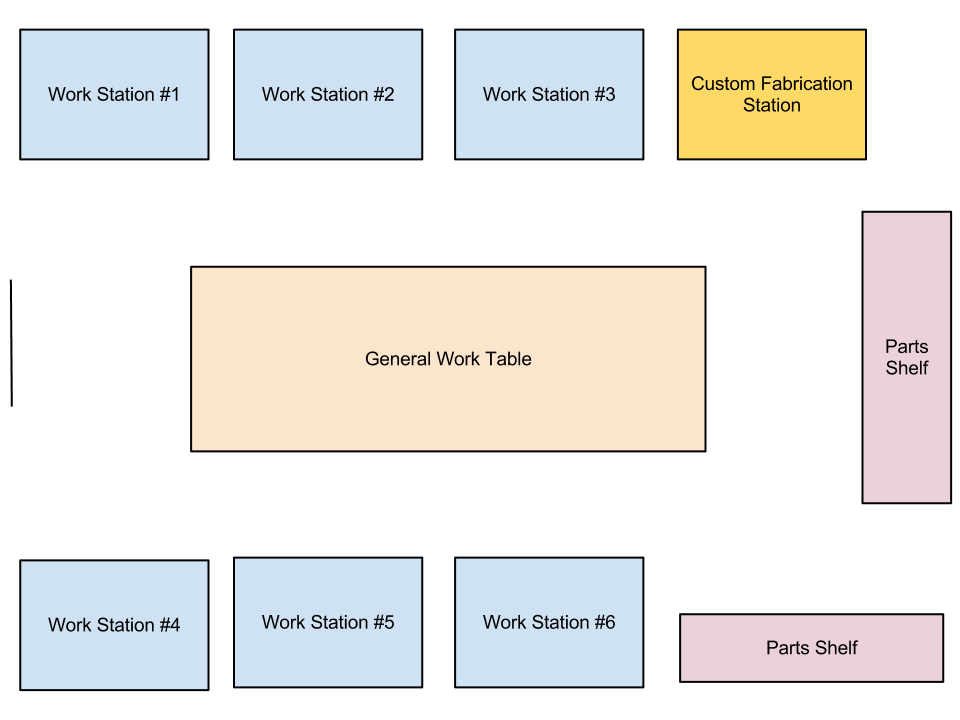
\includegraphics[scale=.4]{images/layout}}
  \label{fig:layout}
  \caption{Layout design of the laboratory}
\end{figure}
\noindent
We designed the lab with ease of use in mind. The room was designed to have room for six workstations, a custom fabrication station, a general work table, and part shelves.  \\

\noindent
Each workstation will have it's own computer preloaded with all the needed software to run the programs. The stations will also be equiped with the necessary equipment to develop and work on embedded devices, such as programmers, simple sensors, resistor/capacitor boxes, hobbiest motors and other actuators along with soldering iron/solder and breadboards. \\

\noindent
The custom fabrication station will be used in the development of custom devices for when a standard board won't work. The station will contain specialized software and equipment for fabrication that the other stations won't have.\\

\noindent
The general work table is reserved for Air Force hobbyest generals. It'll be used when more work space is required, or for holding meetings. By default the general work table shouldn't have anything except for a conference phone.

\subsection{Cost}
\noindent
Budgeting is a major concern for this project. While we don't want cost to get in the way of creativity and design, we still want the price of the lab to be as low as possible. \\

\noindent
Rough estimates are about 10k for the complete lab. 


\subsection{Previous Models}


\subsubsection{A Virtual Embedded Microcontroller Laboratory for Undergraduate Education: Development and Evaluation}
\textit{http://www.edgj.org/index.php/EDGJ/article/view/223} 
\\ \hfill \\
\noindent
Laboratory instruction is a major component of the engineering and technology undergraduate curricula. Traditional laboratory instruction is hampered by several factors including limited access to resources by students and high laboratory maintenance cost. A photorealistic 3D computer-simulated laboratory for undergraduate instruction in microcontroller technology was developed to address these issues. The virtual laboratory includes a realistic representation of devices and components used in a traditional laboratory setting. The virtual laboratory requires the students to engage in the same processes as the traditional laboratory. An initial formative evaluation of the virtual laboratory environment (VLE) was conducted with a group of 42 undergraduate students enrolled in an introductory microcontroller course at Purdue University. Findings show that students perceived the VLE experience comparable to the physical laboratory experience; in addition, they thought the VLE was easy-to use, engaging and useful. In the paper we describe the development of the VLE and report and discuss the results of the evaluation.

\subsubsection{Designing and Implementing a Virtual 3D Microcontroller Laboratory Environment}
\textit{http://ieeexplore.ieee.org/xpl/articleDetails.jsp?reload=true&arnumber=4117022}
\\ \hfill \\ 
\noindent
Laboratory instruction is a major component of undergraduate curriculums throughout the United States. The laboratory experiences represent fundamental instructions for all technology students. Traditional laboratory instruction is hampered by several factors including limited access to resources by students, high laboratory maintenance cost and the inability to delivery the laboratory content of a course at distance. This paper describes the development of an interactive, photorealistic 3D computer-simulated laboratory for undergraduate instruction in microcontroller technology. The virtual lab operates and produces results equal to the physical laboratory. In addition, it includes an extremely realistic representation of devices and components, thus providing the students with the mental engagement necessary to successfully complete the experiments outside the confines of a traditional laboratory. The 3D virtual lab can solve the majority of the problems associated with traditional laboratory instruction, and can provide students with the same level of understanding of the experiments as a real laboratory environment


\subsubsection{Embedded Laboratory}
\textit{https://sites.google.com/site/coolembeddedlaboratory/}
\\ \hfill \\
\noindent
This site aims to teach the students, the well known technical languages like  MATLAB, JAVA , J2EE, HFSS, CST, PSPICE, PCB Designing,mikroC for PIC, MPLAB IDE along with Hi-TECH C Compiler, Keil uVision etc and their practical implementation.

\subsubsection{Embedded Lab}
\textit{http://www.embedded-lab.com/}
\\ \hfill \\
\noindent
Embedded Lab's fully instructional tutorials, experiments and projects will guide you to learn about microcontrollers and embedded systems on your own.

\subsubsection{Embedded Systems and Codesign Laboratory}
\textit{http://codesign.cs.tamu.edu/}
\\ \hfill \\
As the world of engineering advances, the complexity demands of both hardware and software grow at a phenomenal rate. The trade-offs between hardware and software within a system are at the forefront of this complexity and demand attention unto themselves. Hardware software codesign is the study of how to make these tradeoffs and meet system constraints.

\subsubsection{Embedded Systems Laboratory}
\textit{http://esl.epfl.ch/}
\\ \hfill \\
The Embedded Systems Laboratory (ESL) is part of the Institute of Electrical Engineering at EPFL, and focuses on the definition of reliability-aware design, optimization methodologies and system-level exploration tools for high-performance embedded systems and nano-scale multi-processor system-on-chip (MPSoC) architectures.
\end{document}
